\documentclass{beamer}
\usepackage{beamerthemeshadow}
\usepackage[latin1]{inputenc}
\usepackage[english]{babel}
\usepackage{amsmath}
\usepackage{amssymb}
\usepackage{color}
\usepackage{lscape}
\usepackage{alltt}
\usepackage{array}
\usepackage{color}
\usepackage{listings}
\usepackage{graphicx}
\usepackage{csquotes}
\usepackage{caption}
\usepackage{subcaption}
\usepackage{soul}

\setbeamertemplate{footline}[frame number]
\graphicspath{ {images/} }

\begin{document}

% title page
\title{ Neural Ordinary Differential Equations with Julia}
\author{Nicolas Holland}
%\author{Nicolas Holland 尼可老师​}


\frame{\titlepage} 

\frame{\frametitle{Overview}
\begin{enumerate}
\item Theory / Math
\begin{enumerate}
\item ODEs
\item Neural Networks
\item Neural ODEs
\end{enumerate}
\item Julia Packages and Dataset
\item Neural ODE Code and Results
\end{enumerate}
}


\frame{\frametitle{Ordinary Differential Equations}

Let $u(t)$ be function in time, $f$ function describing $u$'s derivative $\frac{\partial u}{\partial t}$, starting at time $t_0$:
\ \\
\begin{minipage}{.5\textwidth}
\begin{align*}
\frac{\partial u}{\partial t} &= f(u(t), t)\\
u(t_0) &= u_0
\end{align*}
with $u_0$ being an initial value.
\end{minipage}%
\begin{minipage}{.5\textwidth}
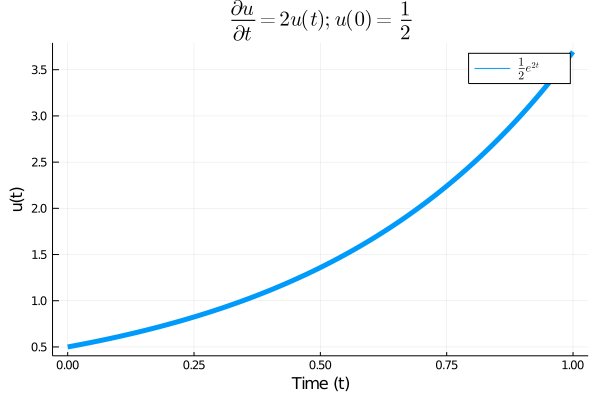
\includegraphics[scale=.3]{ode1}
\end{minipage}
}

\frame{\frametitle{Ordinary Differential Equations}

Let $u(t)$ be function in time, $f$ function describing $u$'s derivative $\frac{\partial u}{\partial t}$, starting at time $t_0$:
\ \\
\begin{minipage}{.5\textwidth}
\begin{align*}
\frac{\partial u}{\partial t} &= f(u(t), t)\\
u(t_0) &= u_0
\end{align*}
with $u_0$ being an initial value.\\ \ \\
Simulate eg. using Euler method:
\begin{align*}
\widetilde{u}_{t+1} = u_{t} + hf(u_{t}, t)
\end{align*}
with $h$ being a step size.
\end{minipage}%
\begin{minipage}{.5\textwidth}
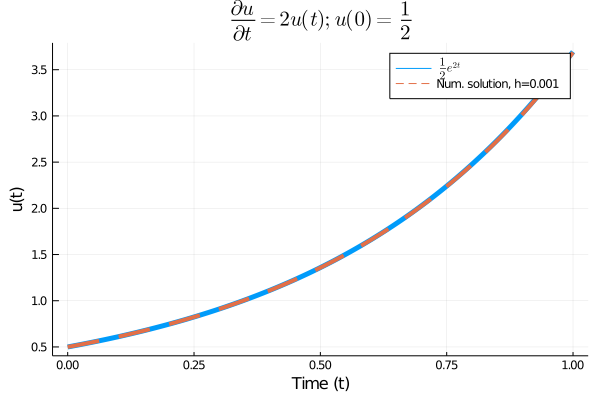
\includegraphics[scale=.3]{ode2}
\end{minipage}
}

\frame{\frametitle{Weather Forecasting}
Numerical Weather Prediction (NWP)
\begin{minipage}{.5\textwidth}
\ \\
\begin{enumerate}
\item PDE (space and time)
\item Modelling of fluid dynamics
\item Navier-Stokes equations
\item Computational heavy
\end{enumerate}
\end{minipage}%
\begin{minipage}{.5\textwidth}
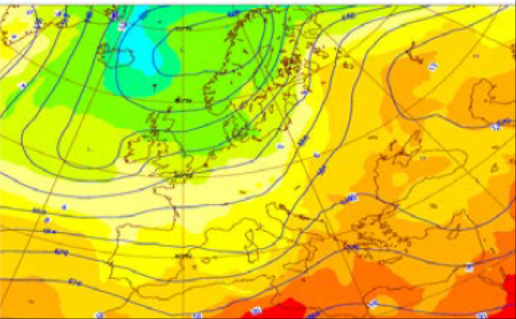
\includegraphics[scale=.3]{nwp}
\end{minipage}

}

\frame{\frametitle{Neural Networks}
Observations

$$u_t, u_{t+1}, u_{t+2}, \cdots$$

}

\frame{\frametitle{Neural Networks}
Observations

$$u_t, u_{t+1}, u_{t+2}, \cdots$$

Can we learn this?

$$ f(u_t, \theta) = u_{t+1} $$

}

\frame{\frametitle{Neural Networks}
Let $f$ be a neural network with $\theta$ being its parameters.
\begin{center}
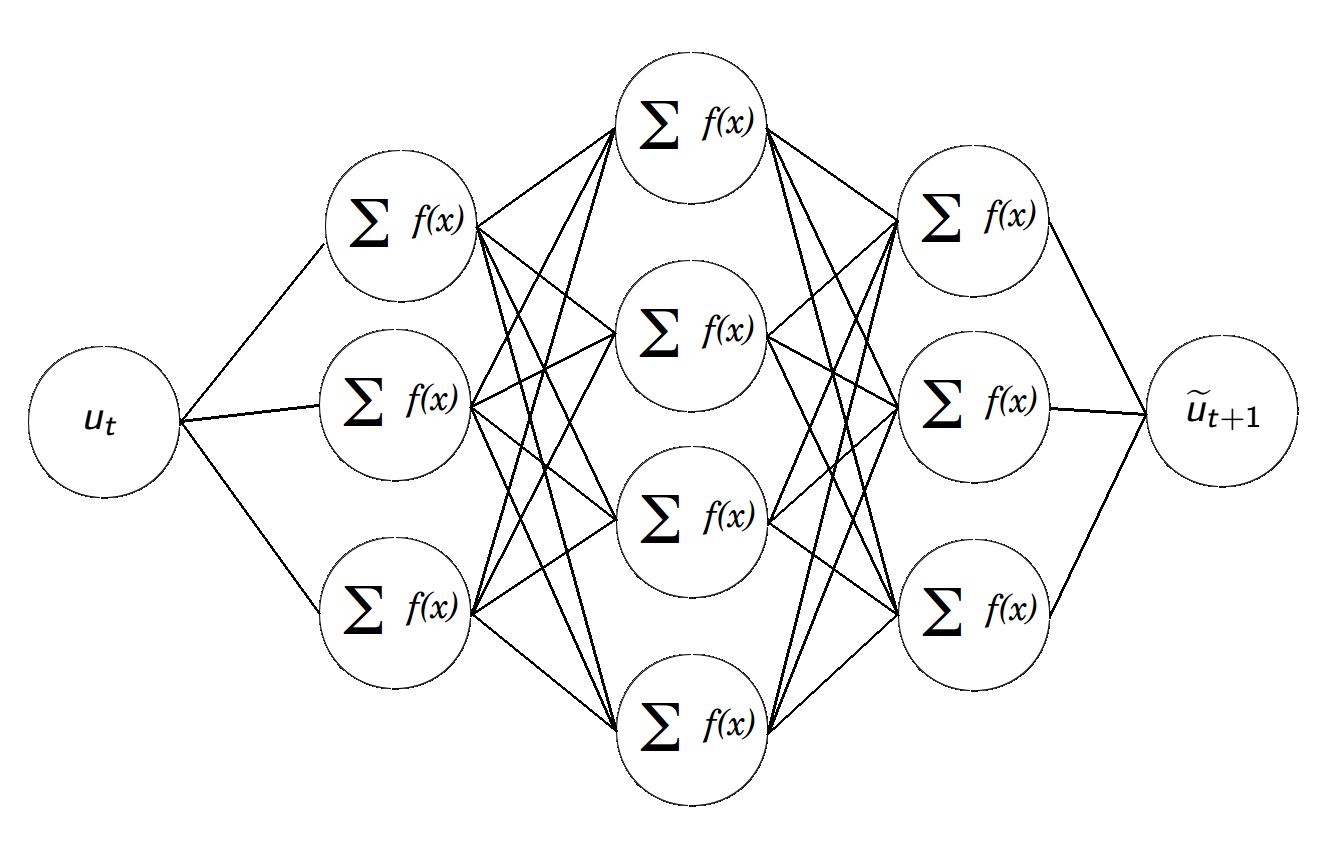
\includegraphics[scale=.21]{network3}
\end{center}
}

\frame{\frametitle{Neural Networks}
Let $f$ be a neural network with $\theta$ being its parameters.
\begin{minipage}{.5\textwidth}
\ \\
\textcolor{green}{Forward} pass:
\begin{align*}
\widetilde{u}_{t+1} = f(u_t, \theta)
\end{align*}
\end{minipage}%
\begin{minipage}{.5\textwidth}
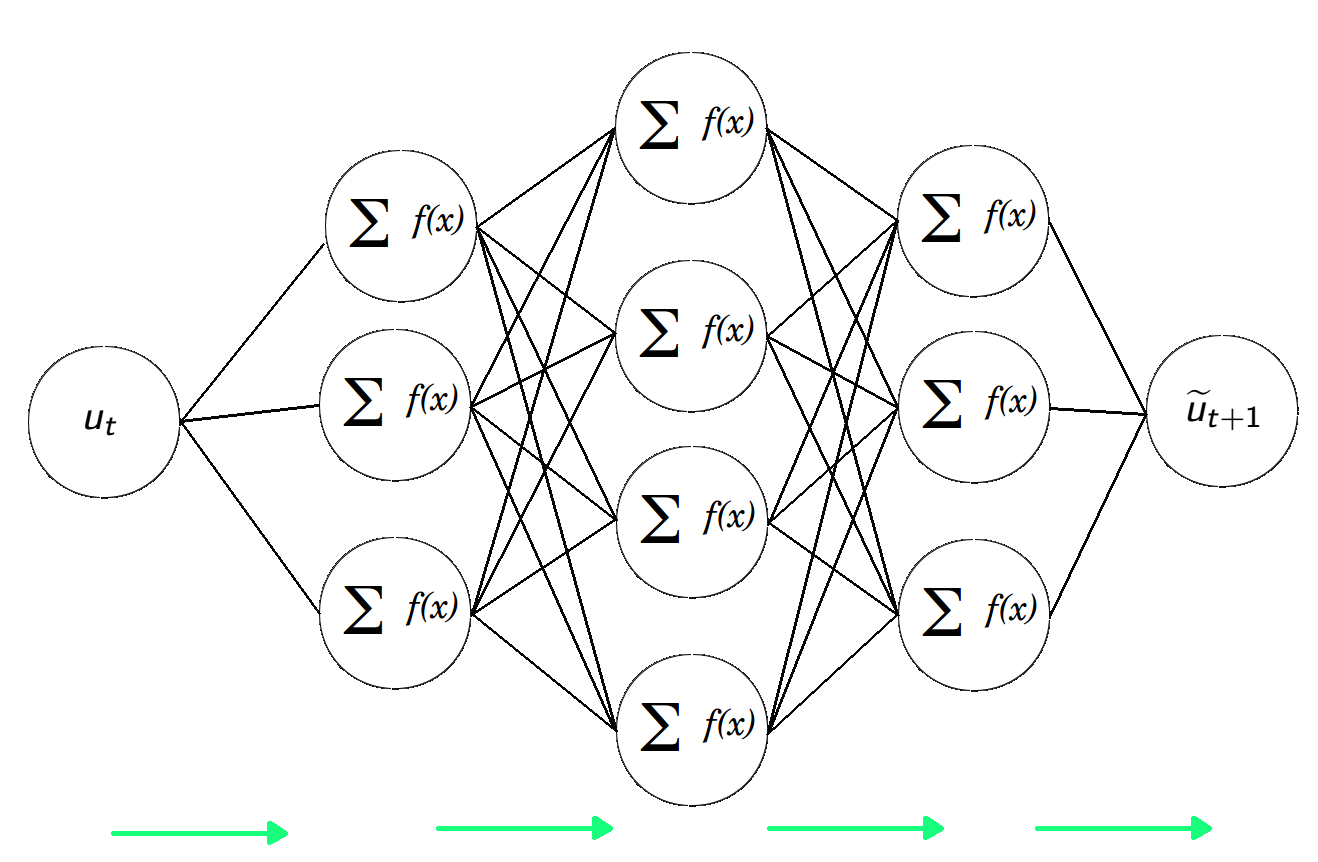
\includegraphics[scale=.21]{network4}
\end{minipage}%
}

\frame{\frametitle{Neural Networks}
Let $f$ be a neural network with $\theta$ being its parameters.
\begin{minipage}{.5\textwidth}
\ \\
Forward pass:
\begin{align*}
\widetilde{u}_{t+1} = f(u_t, \theta)
\end{align*}
\textcolor{red}{Backward} pass:
\begin{align*}
\min_\theta \sum_t\Vert \widetilde{u}_{t} - u_{t} \Vert
\end{align*}
\end{minipage}%
\begin{minipage}{.5\textwidth}
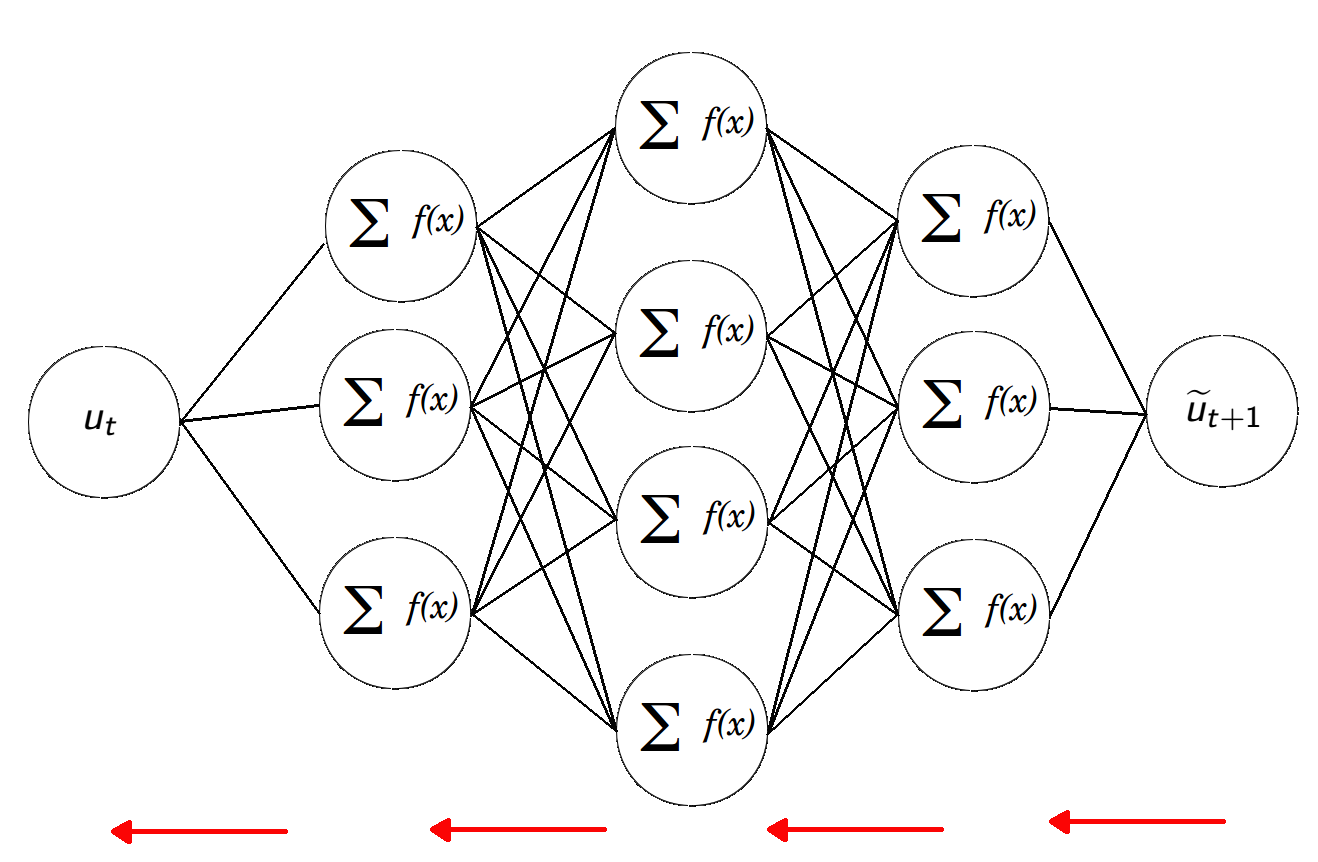
\includegraphics[scale=.21]{network5}
\end{minipage}%
}

\frame{\frametitle{Neural ODEs}
Instead of learning

$$ \widetilde{u}_{t+1} = f(u_t, \theta) $$

we define an ODE 

$$ \frac{\partial u}{\partial t} = f(u(t), t)$$

and learn the change of $u$:

$$ \frac{\partial u}{\partial t} = f(u_t, \theta)$$

}

\frame{\frametitle{Neural ODEs}
Neural ODE:

$$ \frac{\partial u}{\partial t} = f(u_t, \theta)$$

Forward pass:

$$ \widetilde{u}_{t+1} = u_t + h\ \underbrace{f(u_t, \theta)}_{\text{NNs forward pass}} $$

}

\frame{\frametitle{Neural ODEs}
Neural ODE:

$$ \frac{\partial u}{\partial t} = f(u_t, \theta)$$

Forward pass:

$$ \widetilde{u}_{t+1} = u_t + h\ \underbrace{f(u_t, \theta)}_{\text{NNs forward pass}} $$

Backward pass:

$$ \min_\theta \sum_t \Vert \widetilde{u}_{t+1} - u_{t+1} \Vert$$

}

\frame{\frametitle{Neural ODEs}
Neural ODE:

$$ \frac{\partial u}{\partial t} = f(u_t, \theta)$$

Forward pass:

$$ \widetilde{u}_{t+1} = u_t + h f(u_t, \theta) $$


Backward pass:

$$ \min_\theta \sum_t \Vert u_t + h f(u_t, \theta) - u_{t+1} \Vert$$

}

\frame{\frametitle{Neural ODEs}
Neural ODE:

$$ \frac{\partial u}{\partial t} = f(u_t, \theta)$$

Forward pass:

$$ \widetilde{u}_{t+1} = u_t + h f(u_t, \theta) $$

Backward pass (two steps):

$$ \min_\theta \sum_t \Vert \textcolor{blue}{u_t + hf(u_t, \theta)} + hf(\textcolor{blue}{u_t + hf(u_t, \theta)},\theta) - u_{t+2} \Vert$$

}

\frame{\frametitle{Overview}
\begin{enumerate}
\item \st{Theory / Math}
\begin{enumerate}
\item \st{ODEs}
\item \st{Neural Networks}
\item \st{Neural ODEs}
\end{enumerate}
\item Julia Packages and Dataset
\item Neural ODE Code and Results
\end{enumerate}
}


\frame{\frametitle{Julia Packages}
\begin{center}
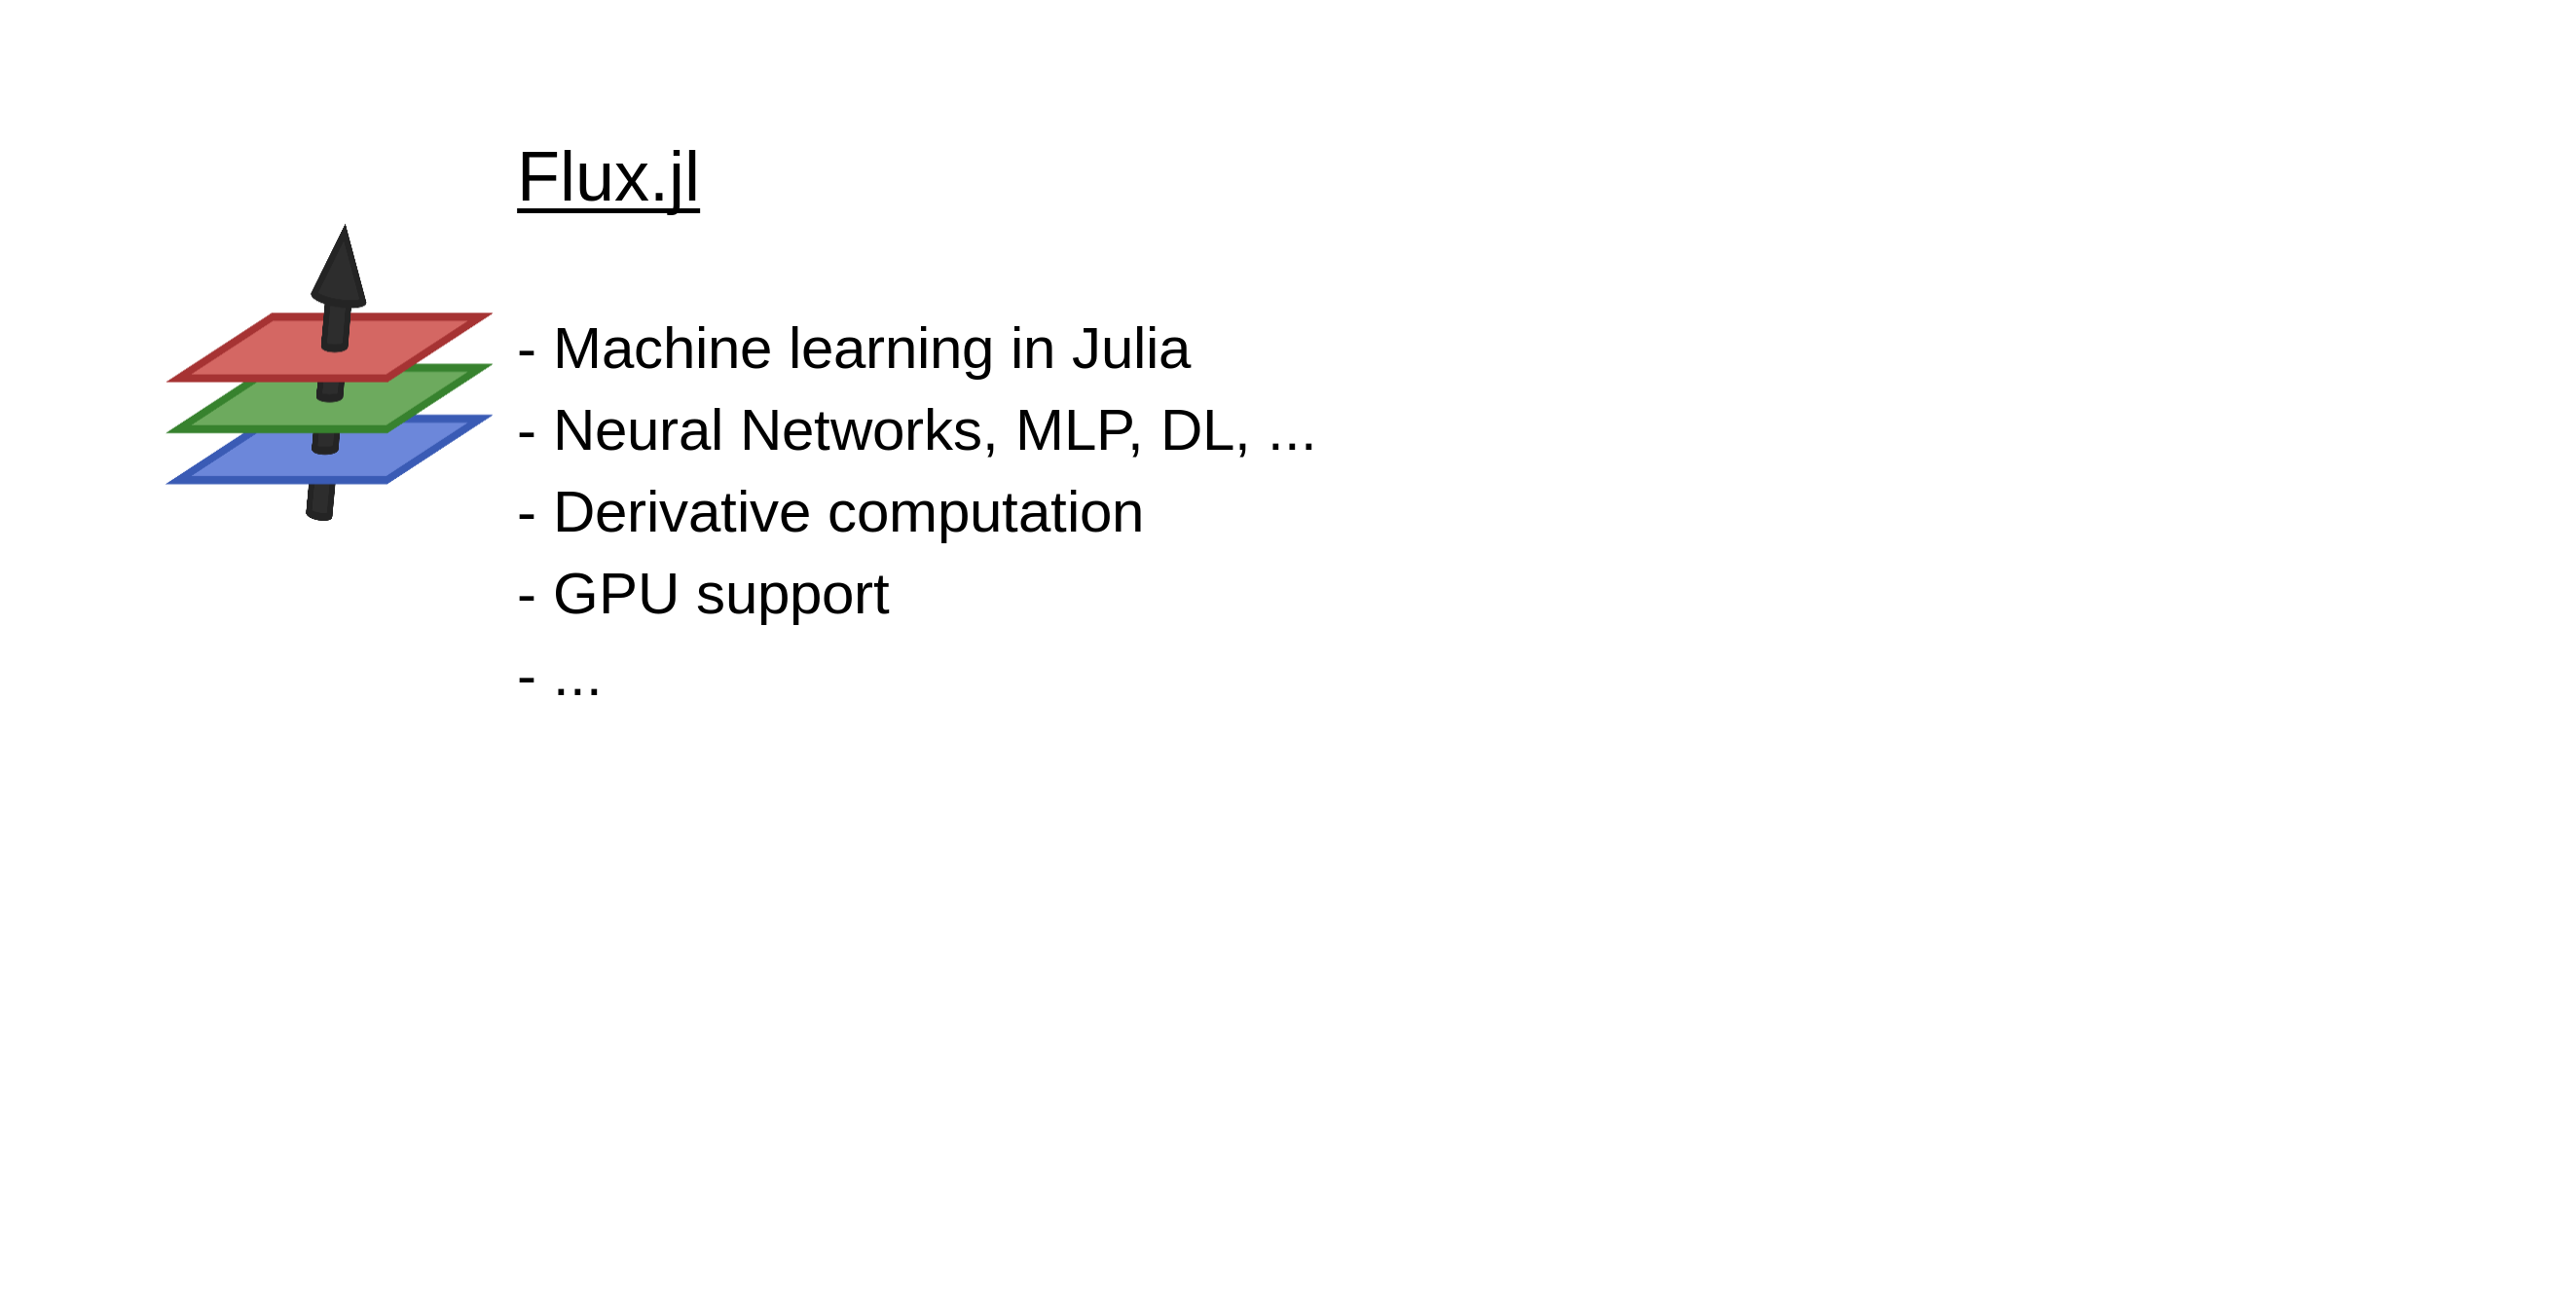
\includegraphics[scale=.12]{package1}
\end{center}
}

\frame{\frametitle{Julia Packages}
\begin{center}
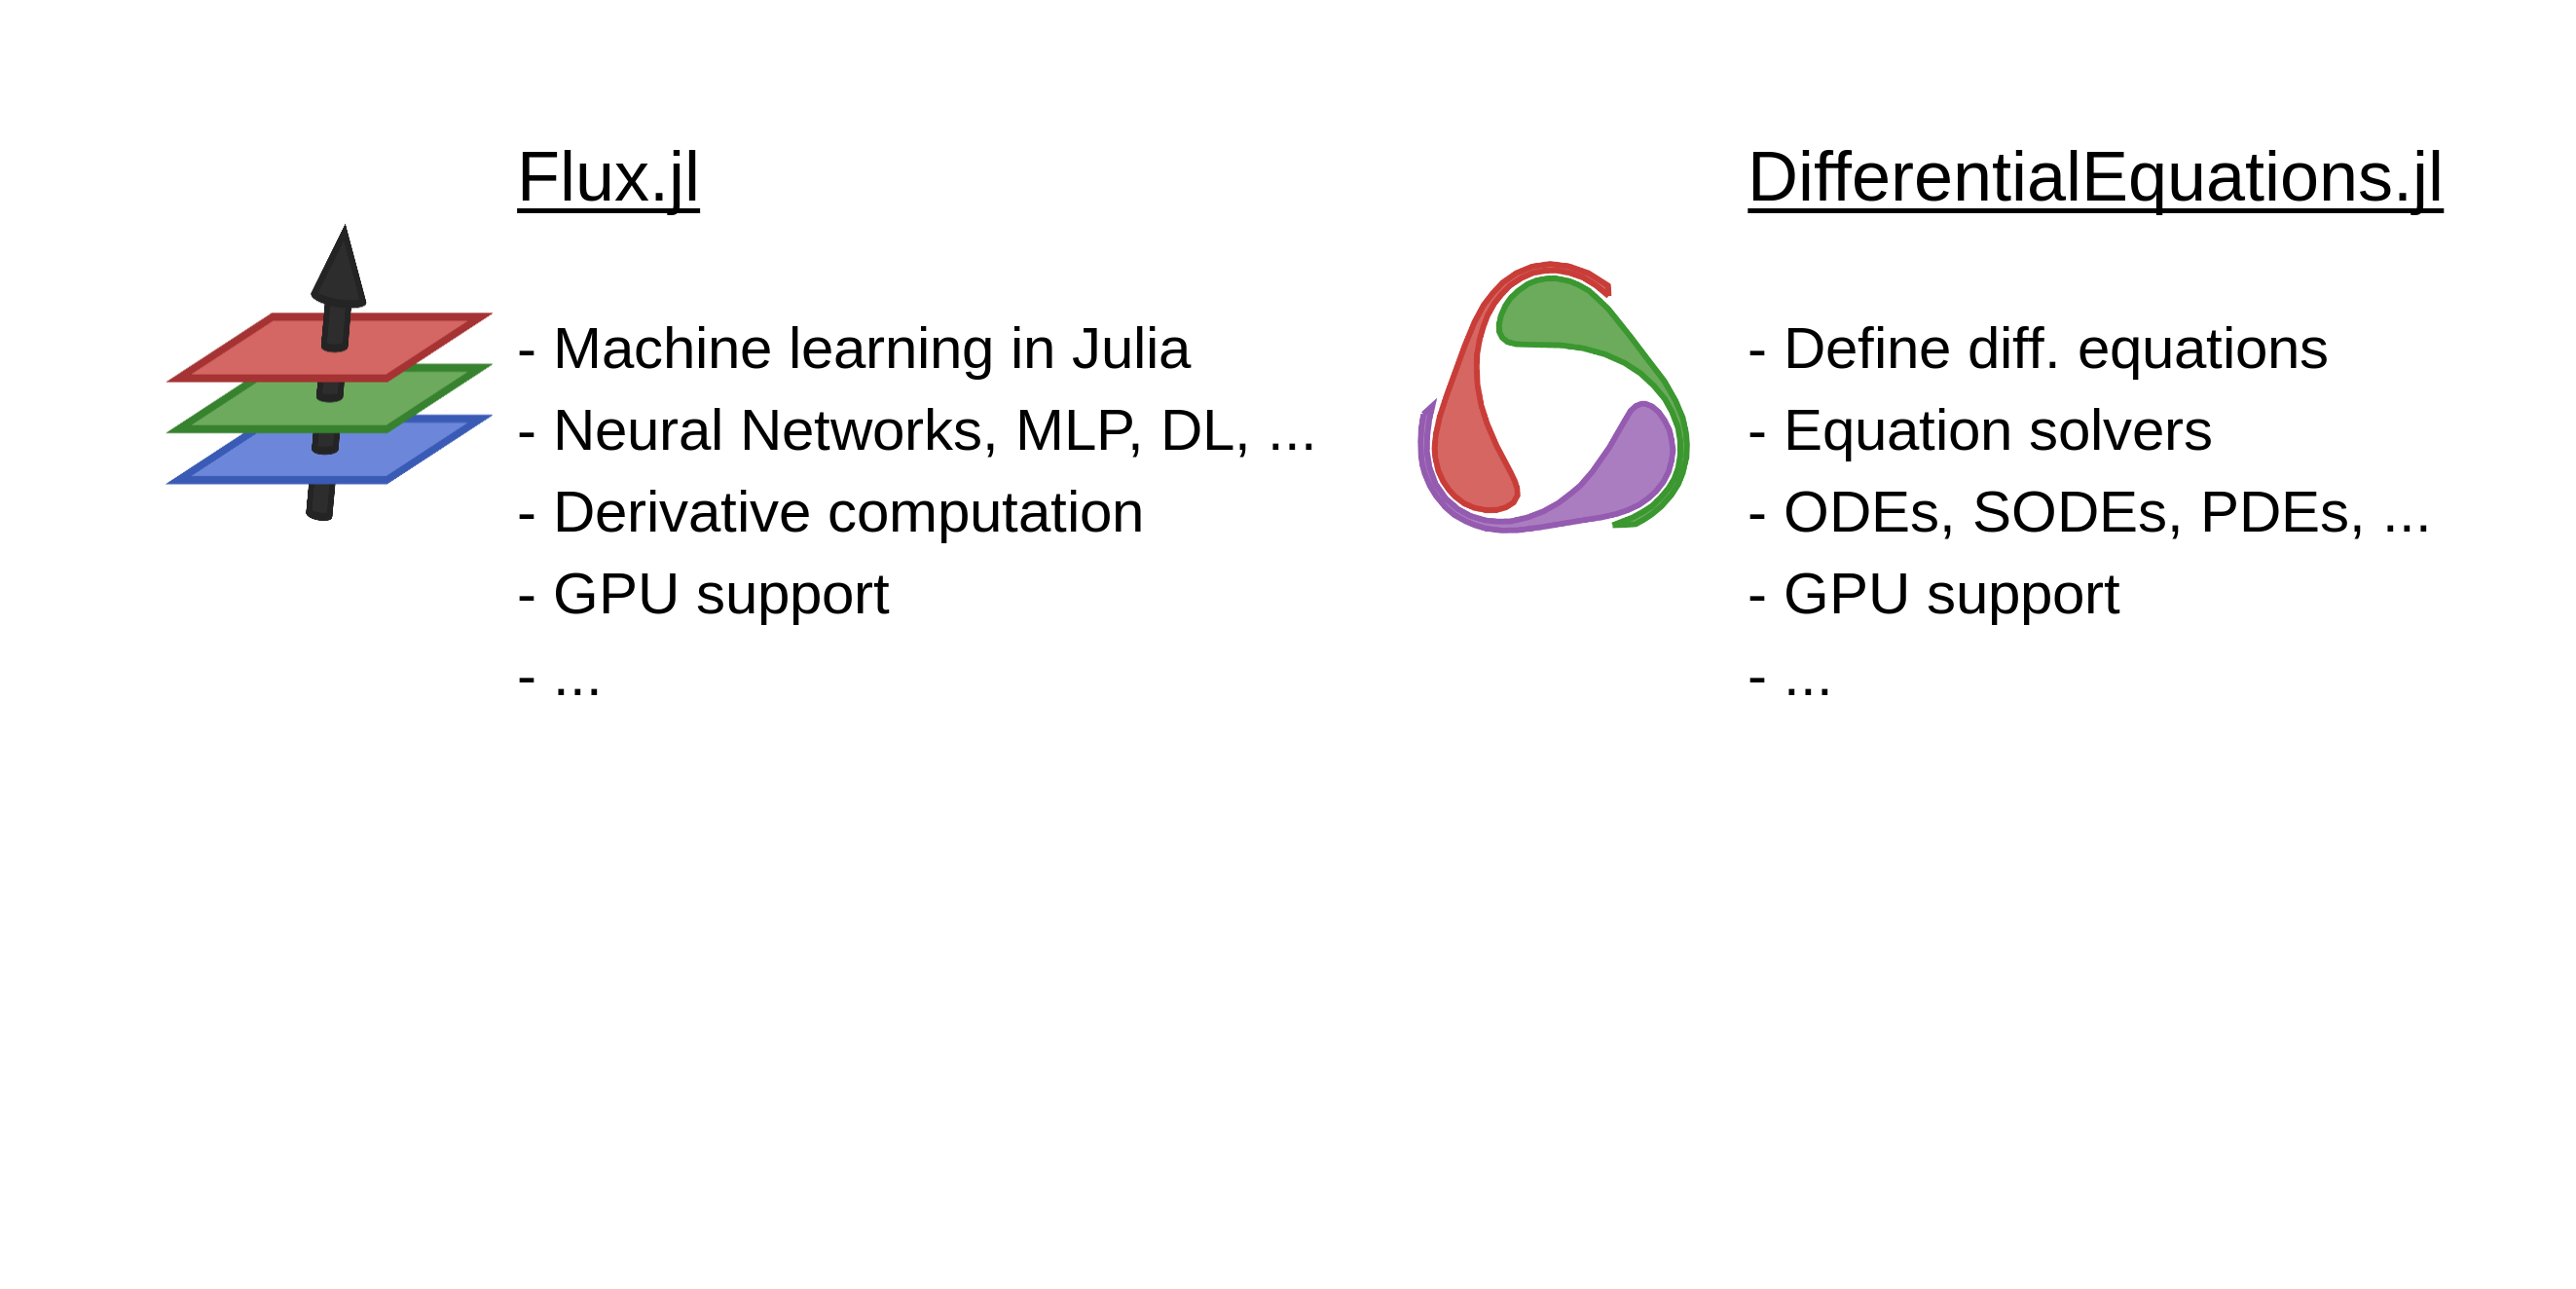
\includegraphics[scale=.12]{package2}
\end{center}
}


\frame{\frametitle{Julia Packages}
\begin{center}
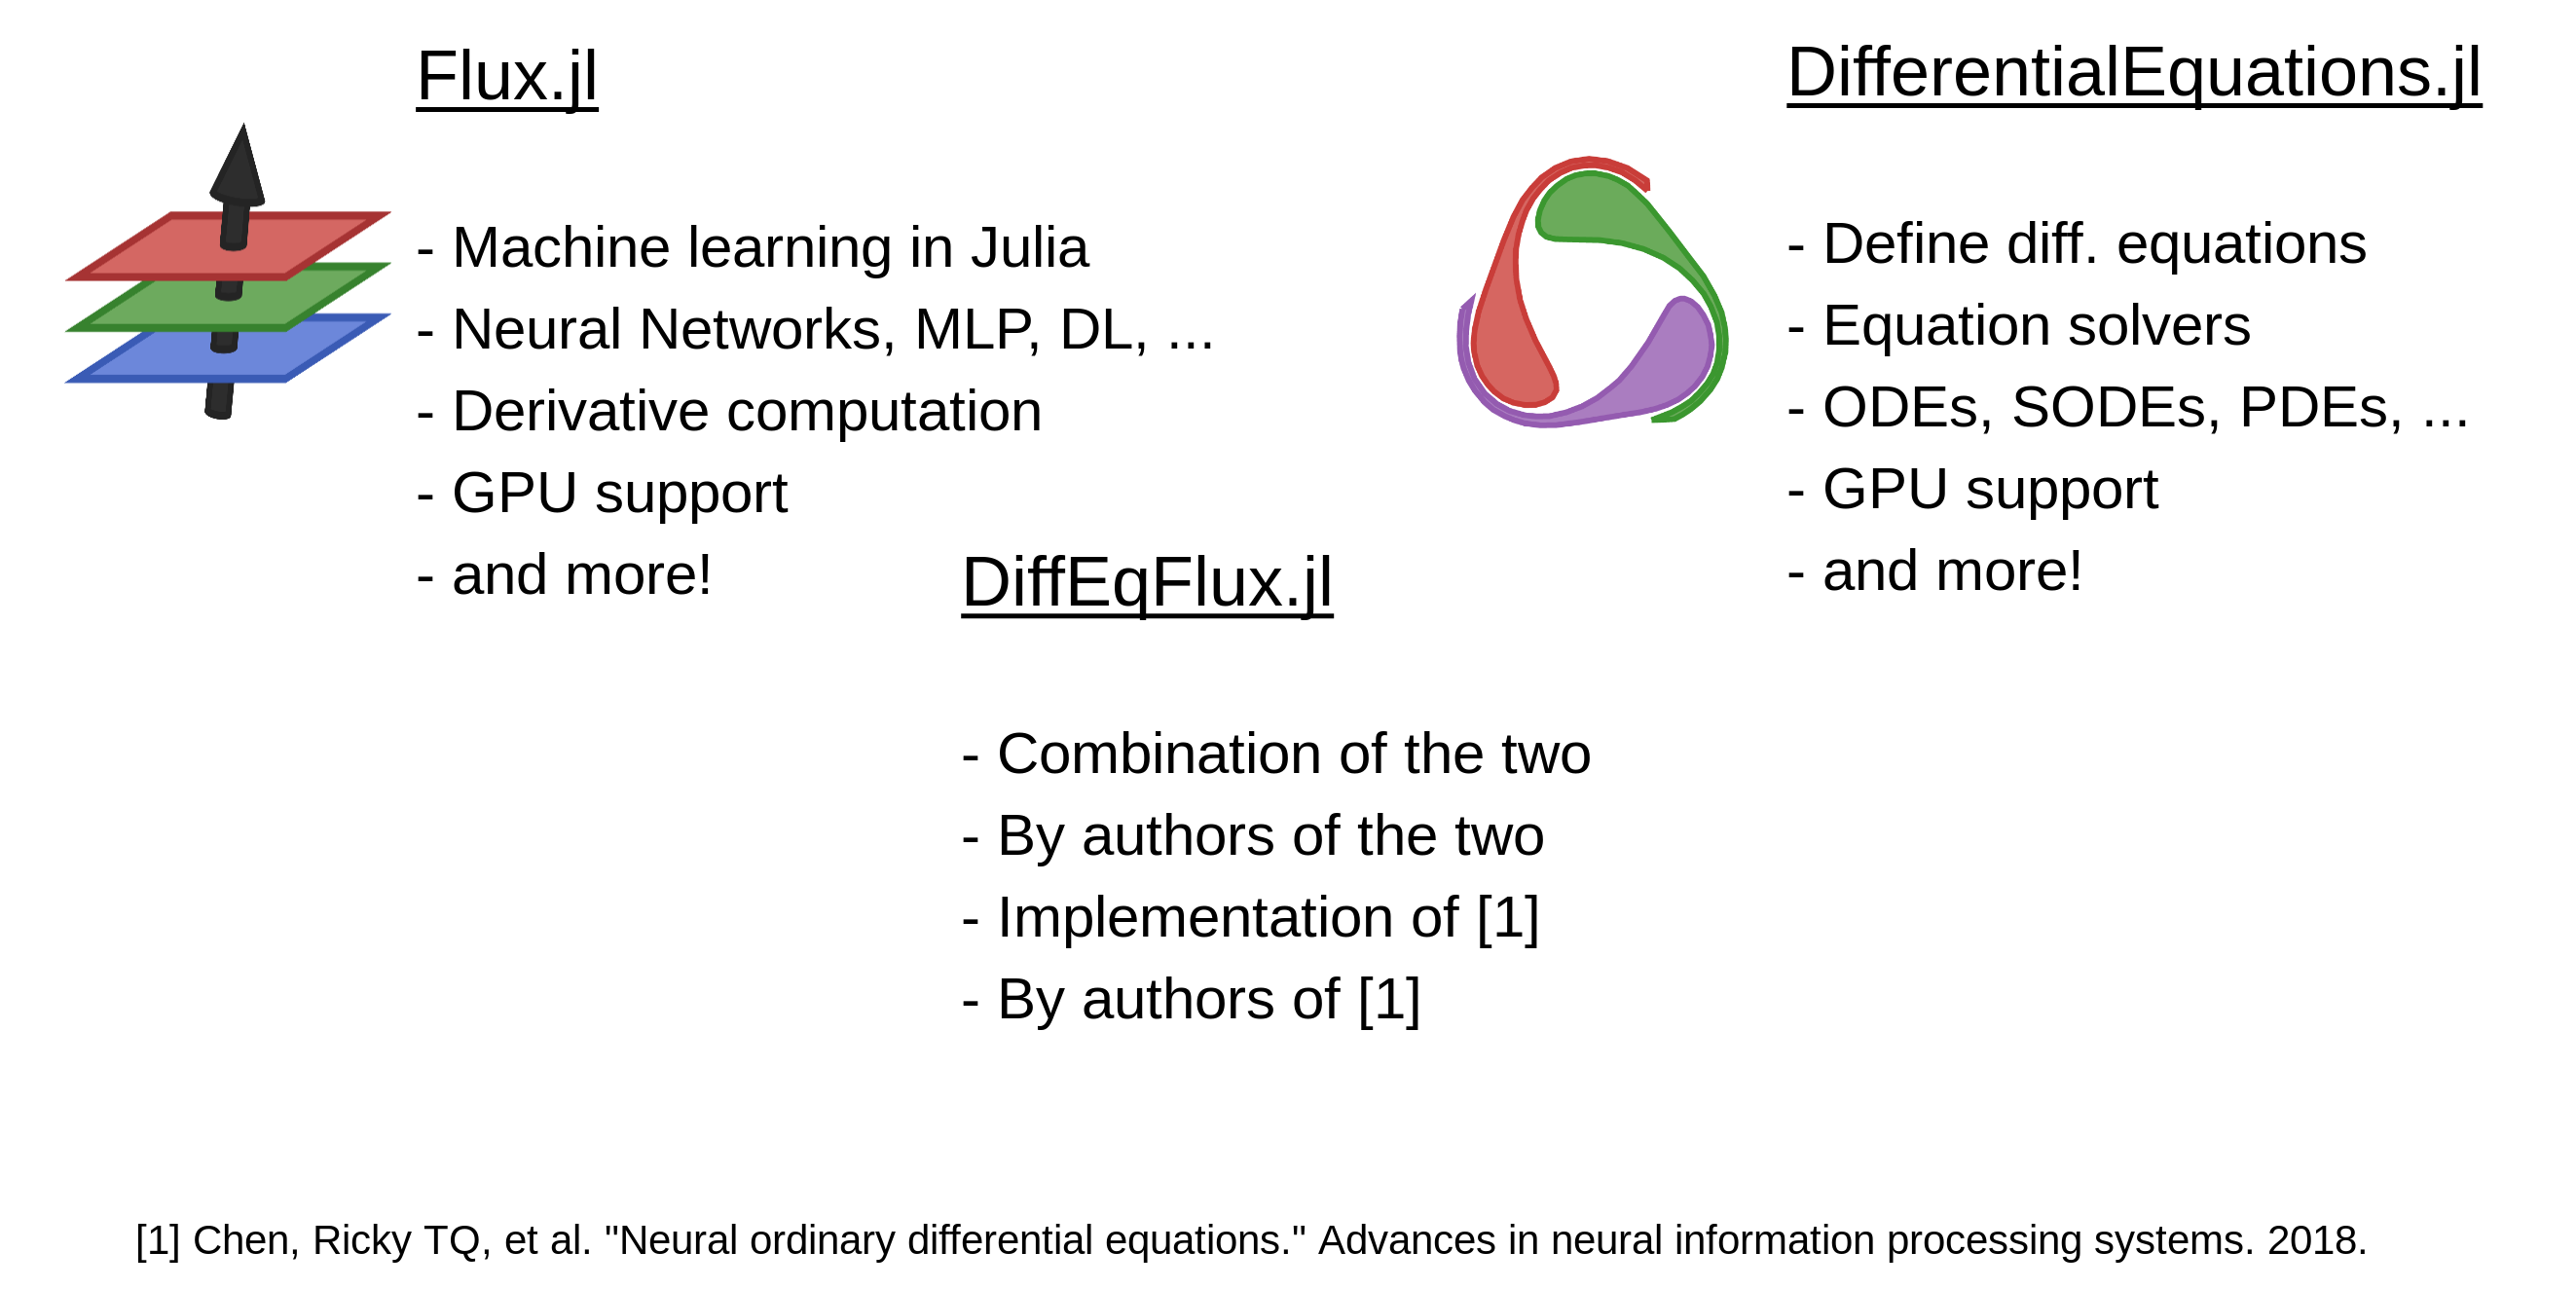
\includegraphics[scale=.12]{package3}
\end{center}
}


\frame{\frametitle{Dataset}
Daily climate data in the city of Delhi from 2013 to 2017.
Includes mean temperature, humidity, wind speed, mean air pressure.\\
\ \\
\begin{minipage}{.5\textwidth}
\centering
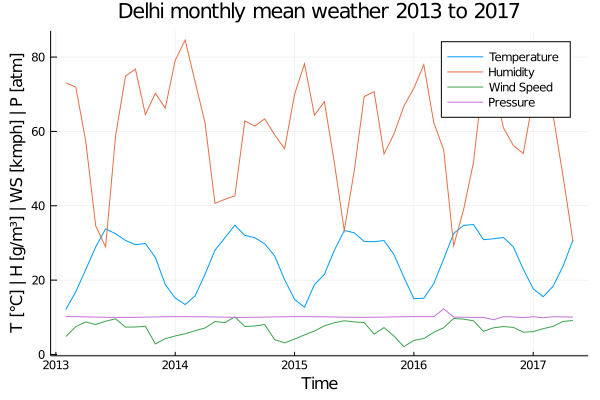
\includegraphics[scale=0.25]{delhi_weather}
\end{minipage}%
\begin{minipage}{.5\textwidth}
\centering
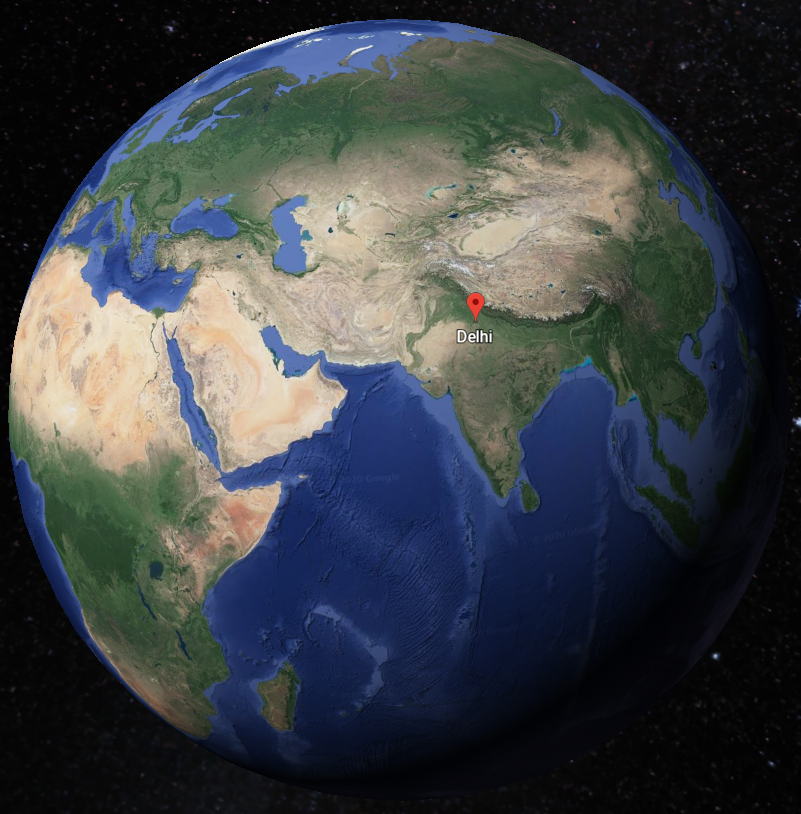
\includegraphics[scale=0.17]{delhi}
\end{minipage}%
}

\frame{\frametitle{Julia Code}
\begin{center}
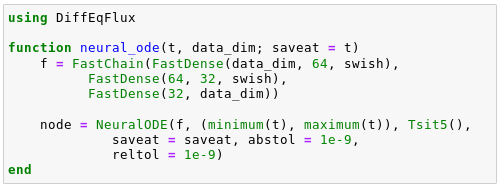
\includegraphics[scale=.6]{code1}
\end{center}
}

\frame{\frametitle{Julia Code}
\begin{center}
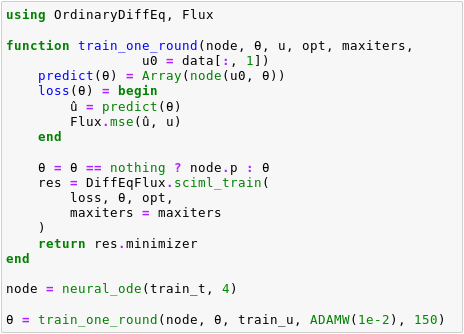
\includegraphics[scale=.6]{code2}
\end{center}
}


\frame{\frametitle{Results}
\begin{center}
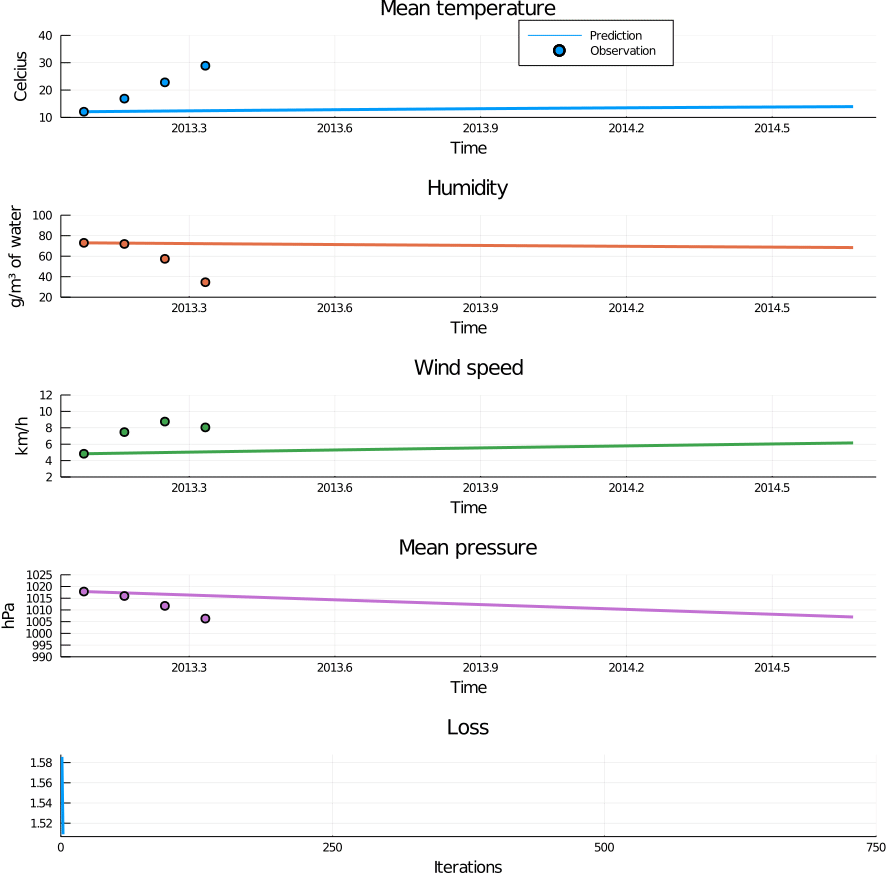
\includegraphics[scale=.25]{result0}
\end{center}
}

\frame{\frametitle{Results}
\begin{center}
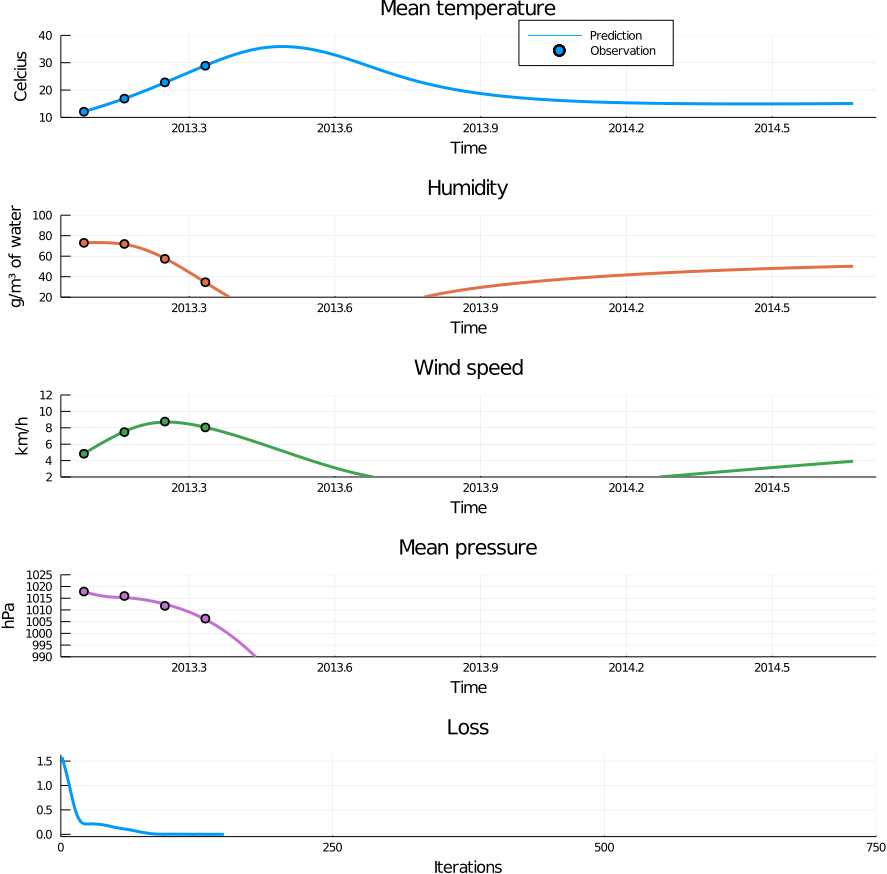
\includegraphics[scale=.25]{result1}
\end{center}
}

\frame{\frametitle{Results}
\begin{center}
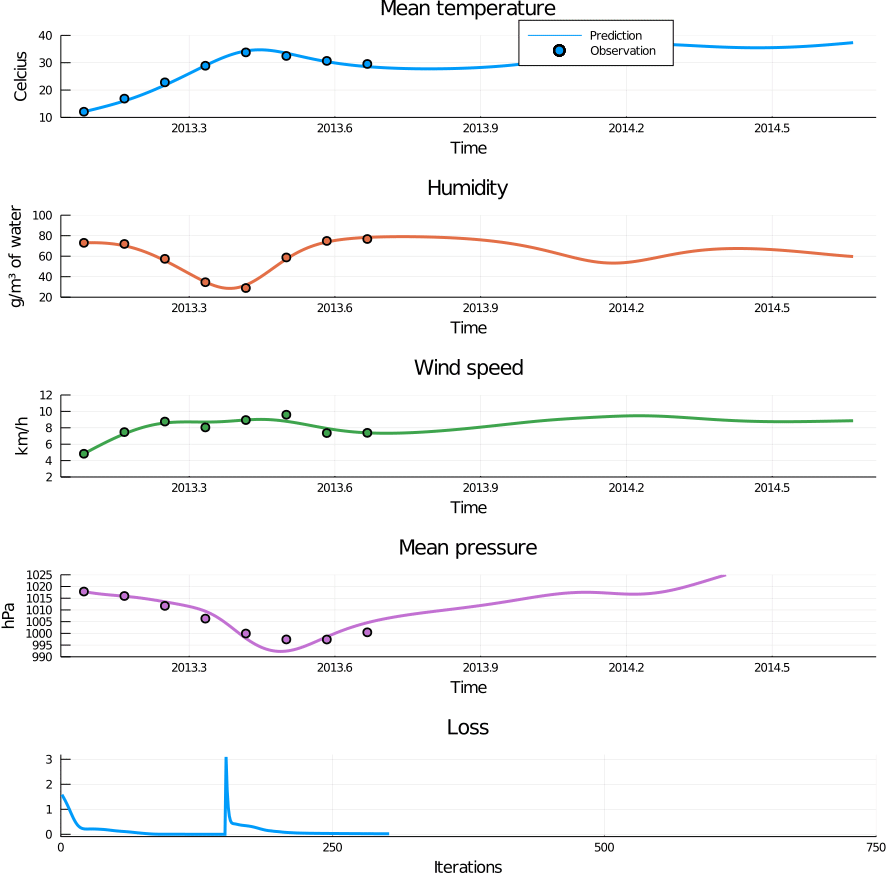
\includegraphics[scale=.25]{result2}
\end{center}
}

\frame{\frametitle{Results}
\begin{center}
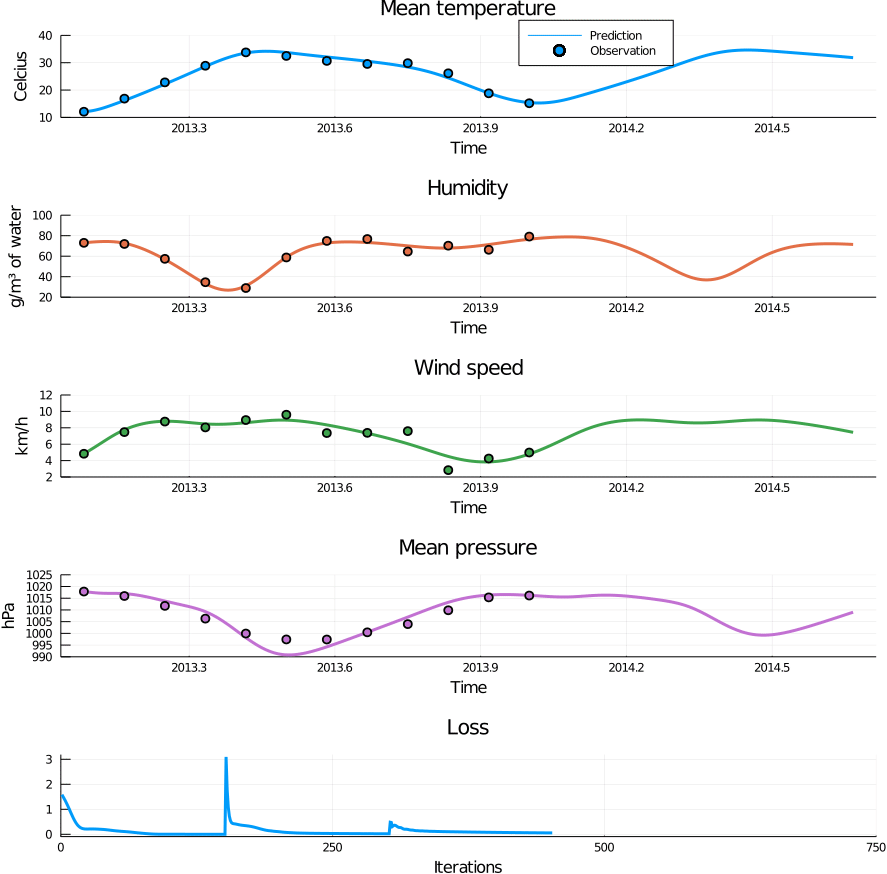
\includegraphics[scale=.25]{result3}
\end{center}
}

\frame{\frametitle{Results}
\begin{center}
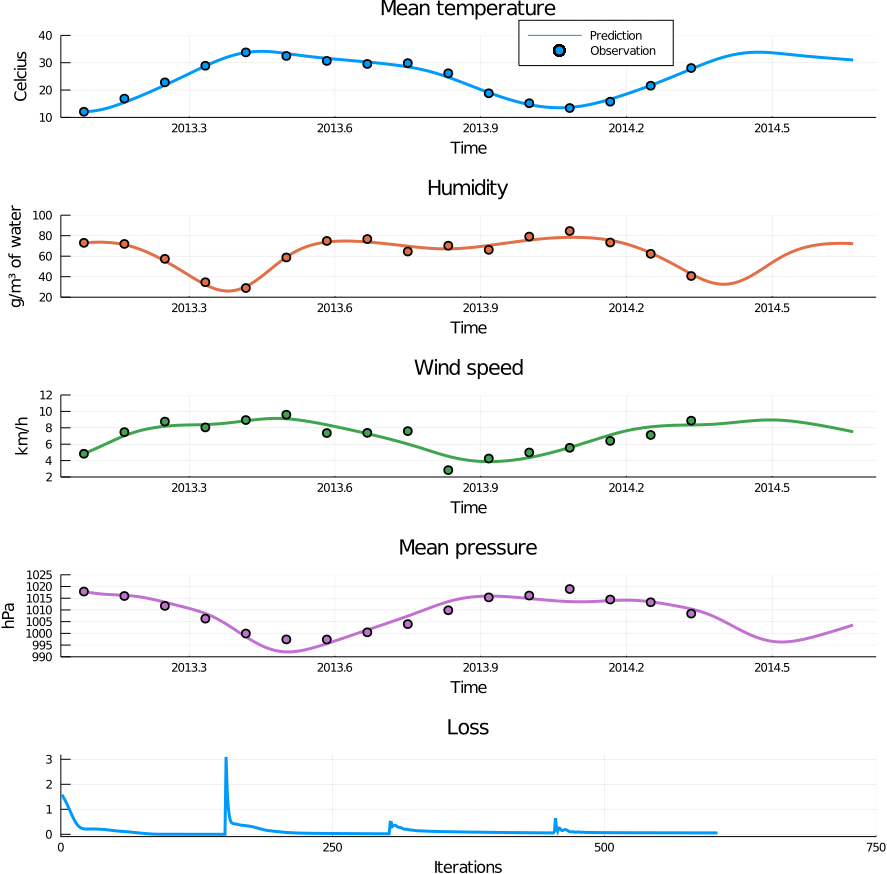
\includegraphics[scale=.25]{result4}
\end{center}
}

\frame{\frametitle{Results}
\begin{center}
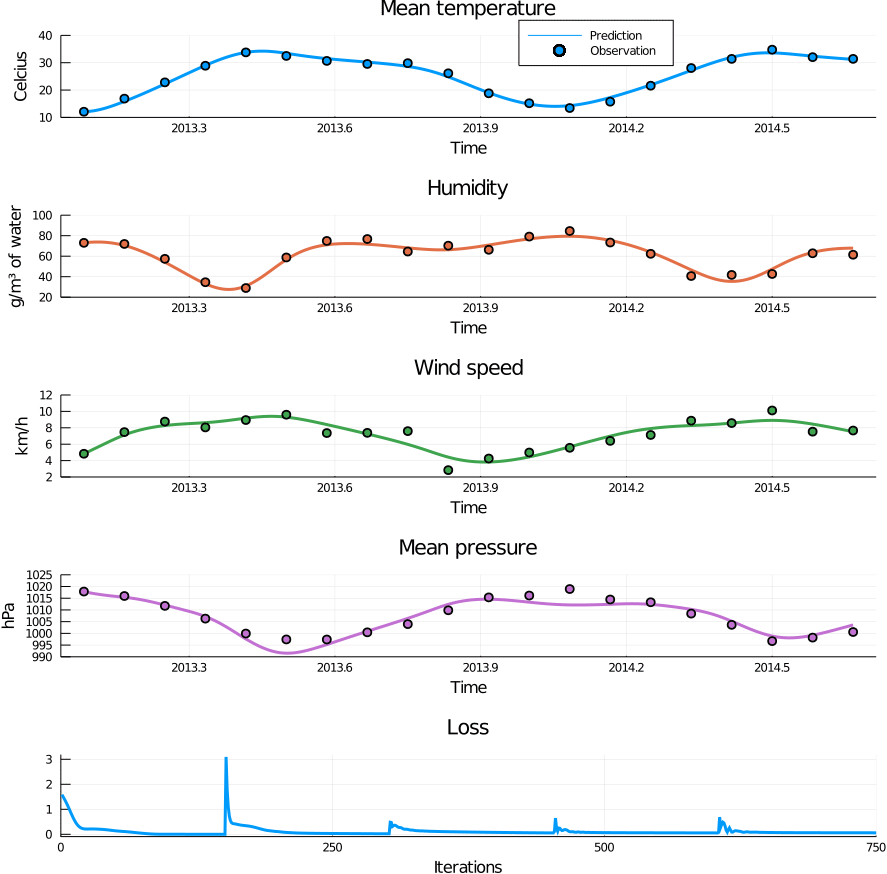
\includegraphics[scale=.25]{result5}
\end{center}
}

\frame{\frametitle{Results}
\begin{center}
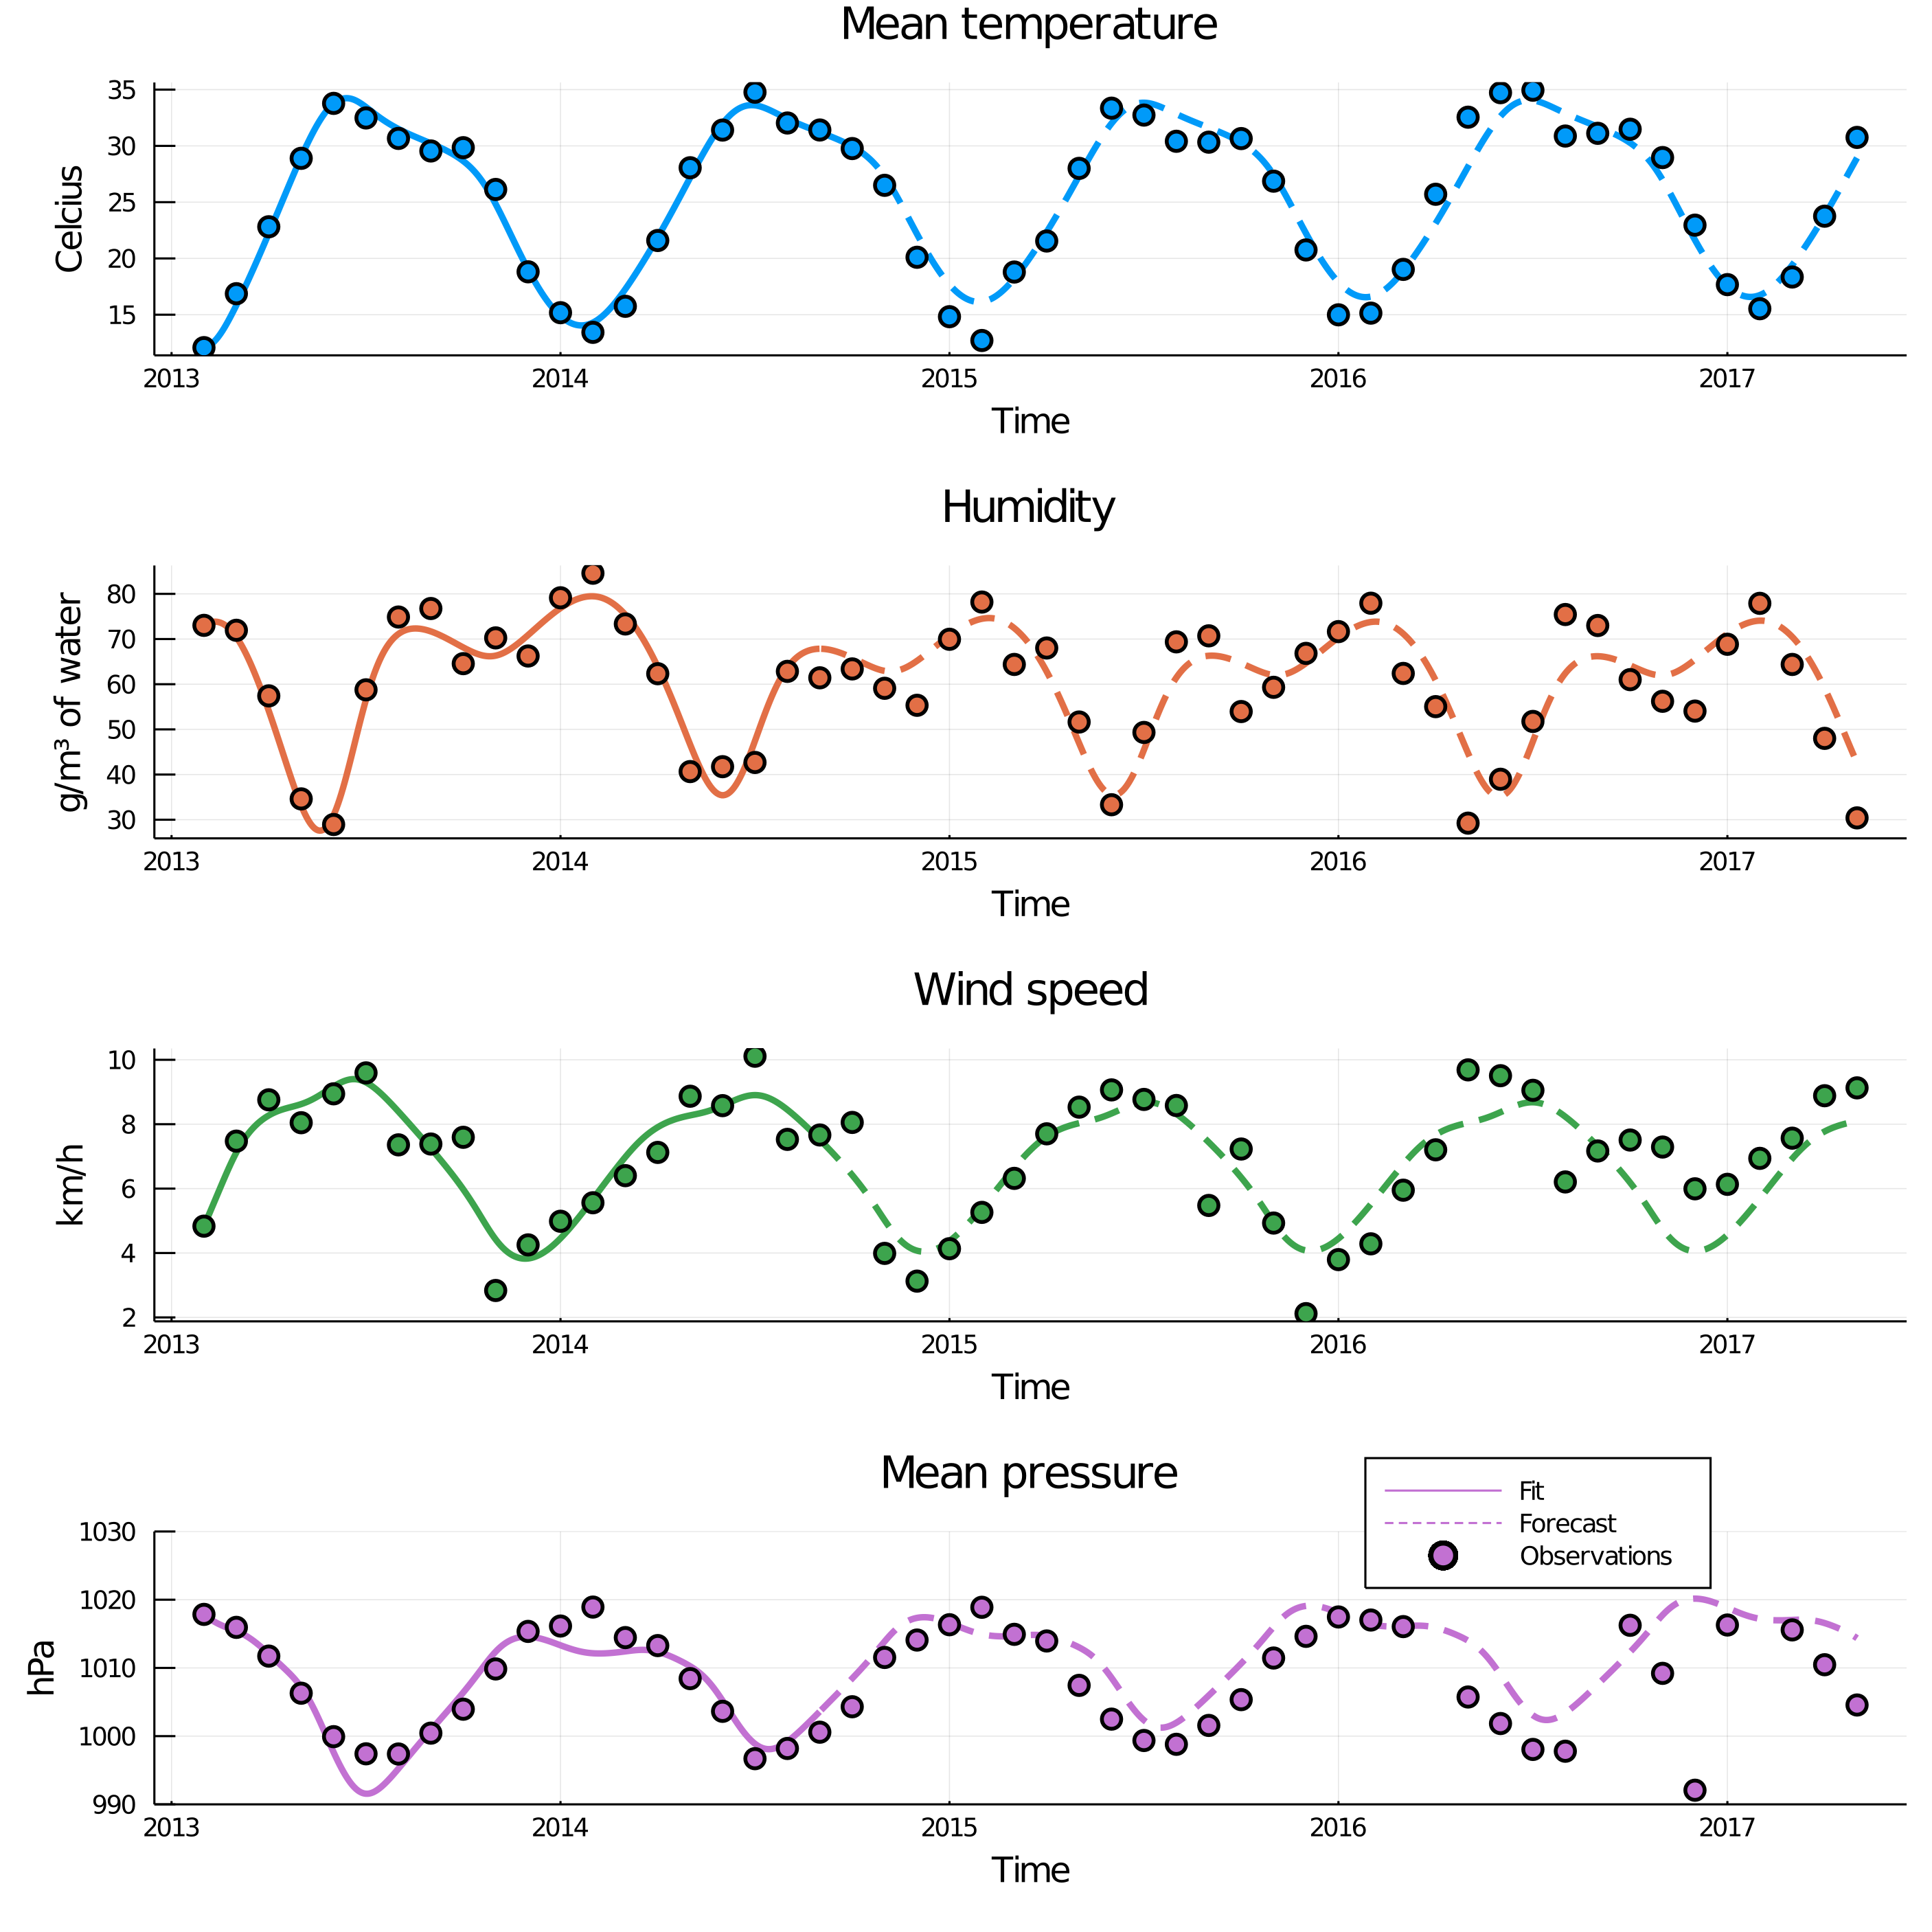
\includegraphics[scale=.3]{result6}
\end{center}
}

\frame{\frametitle{References}
\begin{enumerate}

\item \scriptsize Chen, Ricky TQ, et al. "Neural ordinary differential equations." Advances in neural information processing systems. 2018.
\item  DiffEqFlux Package\\
https://github.com/SciML/DifferentialEquations.jl
\item DiffEqFlux Paper\\
Chris Rackauckas et al. "DiffEqFlux.jl - A Julia Library for Neural Differential Equations", arXiv:1902.02376
\item Original Blog post this talk is based on\\
sebastiancallh.github.io/post/neural-ode-weather-forecast/
\item Link to talk + my code\\
github.com/nicolasholland/VariousProjects/tree/master/Neural ODE Talk
\item kaggel dataset\\
www.kaggle.com/sumanthvrao/daily-climate-time-series-data
\end{enumerate}
}

\end{document}